\chapter{Attack Design}

In this section, we describe the design of our automatic feature generation model, outline the attack strategy and explain certain design decisions.
Most of this section will be split into two different sections.
First we describe the feature generation process and then the overall attack.

\section{Stacked Autoencoder}

A stacked autoencoder takes a fixed-length input vector and tries to learn a function that compresses that vector.
Thus if we were to use it for our fingerprinting extraction model, we will need to preprocess the variable-length traces into a fixed-length input.
There are various different manners of doing this.
One of the most naive ones is to find the longest length trace and pad all of the other traces up to that length.
However, in Greschbach et al.'s dataset, this length is around $250,000$ \cite{greschbach2016effect}, which means that our network will need to be incredibly deep to extract a short trace.

Instead, we pick the average length of the traces, which is around $3,000$ and cut or pad traces which are longer or shorter.
On top of that, we deal with the fact that each packet is represented by a tuple, by just multiplying the time by the direction.
Therefore, all of the outgoing packets are positive whilst the incoming ones will be negative.

\section{Sequence-to-Sequence Model}

As described in section \ref{sec:seq2seq}, a sequence-to-sequence model is able to learn how to construct a fixed-length representation from a variable-length sequence, which means that we will not have to perform as much preprocessing as for our autoencoder.

Although we already know the overall structure, there are still a couple of design decisions that had to be made specifically for our attack.
These decisions are outlined in the following section.

One of the parameters which we will examine first is the \textit{amount of hidden states} in the RNN cells.
This number affects the amount of neurons for each layer with the cells.
Hence, if for example the amount of hidden neurons is set to $100$, the state with an LSTM cell is represented by vector of length $200$ (since the state is represented by two vectors of length $100$).
The higher this number, the easier it should be to learn a representation, as the compression factor is lower.
But we also need to consider the fact that the higher the amount of hidden neurons, the more variables the model needs to learn and thus the more complex the computations are.

Each value in a trace can be represented by a vector of length two (timestamp and direction), as seen in table \ref{table:cell-extract}.
Therefore, if the amount of hidden cells is not equal to two, we will also need to \textit{project} the input and output to the necessary dimensions.

\begin{figure}[ht]
  \centering
  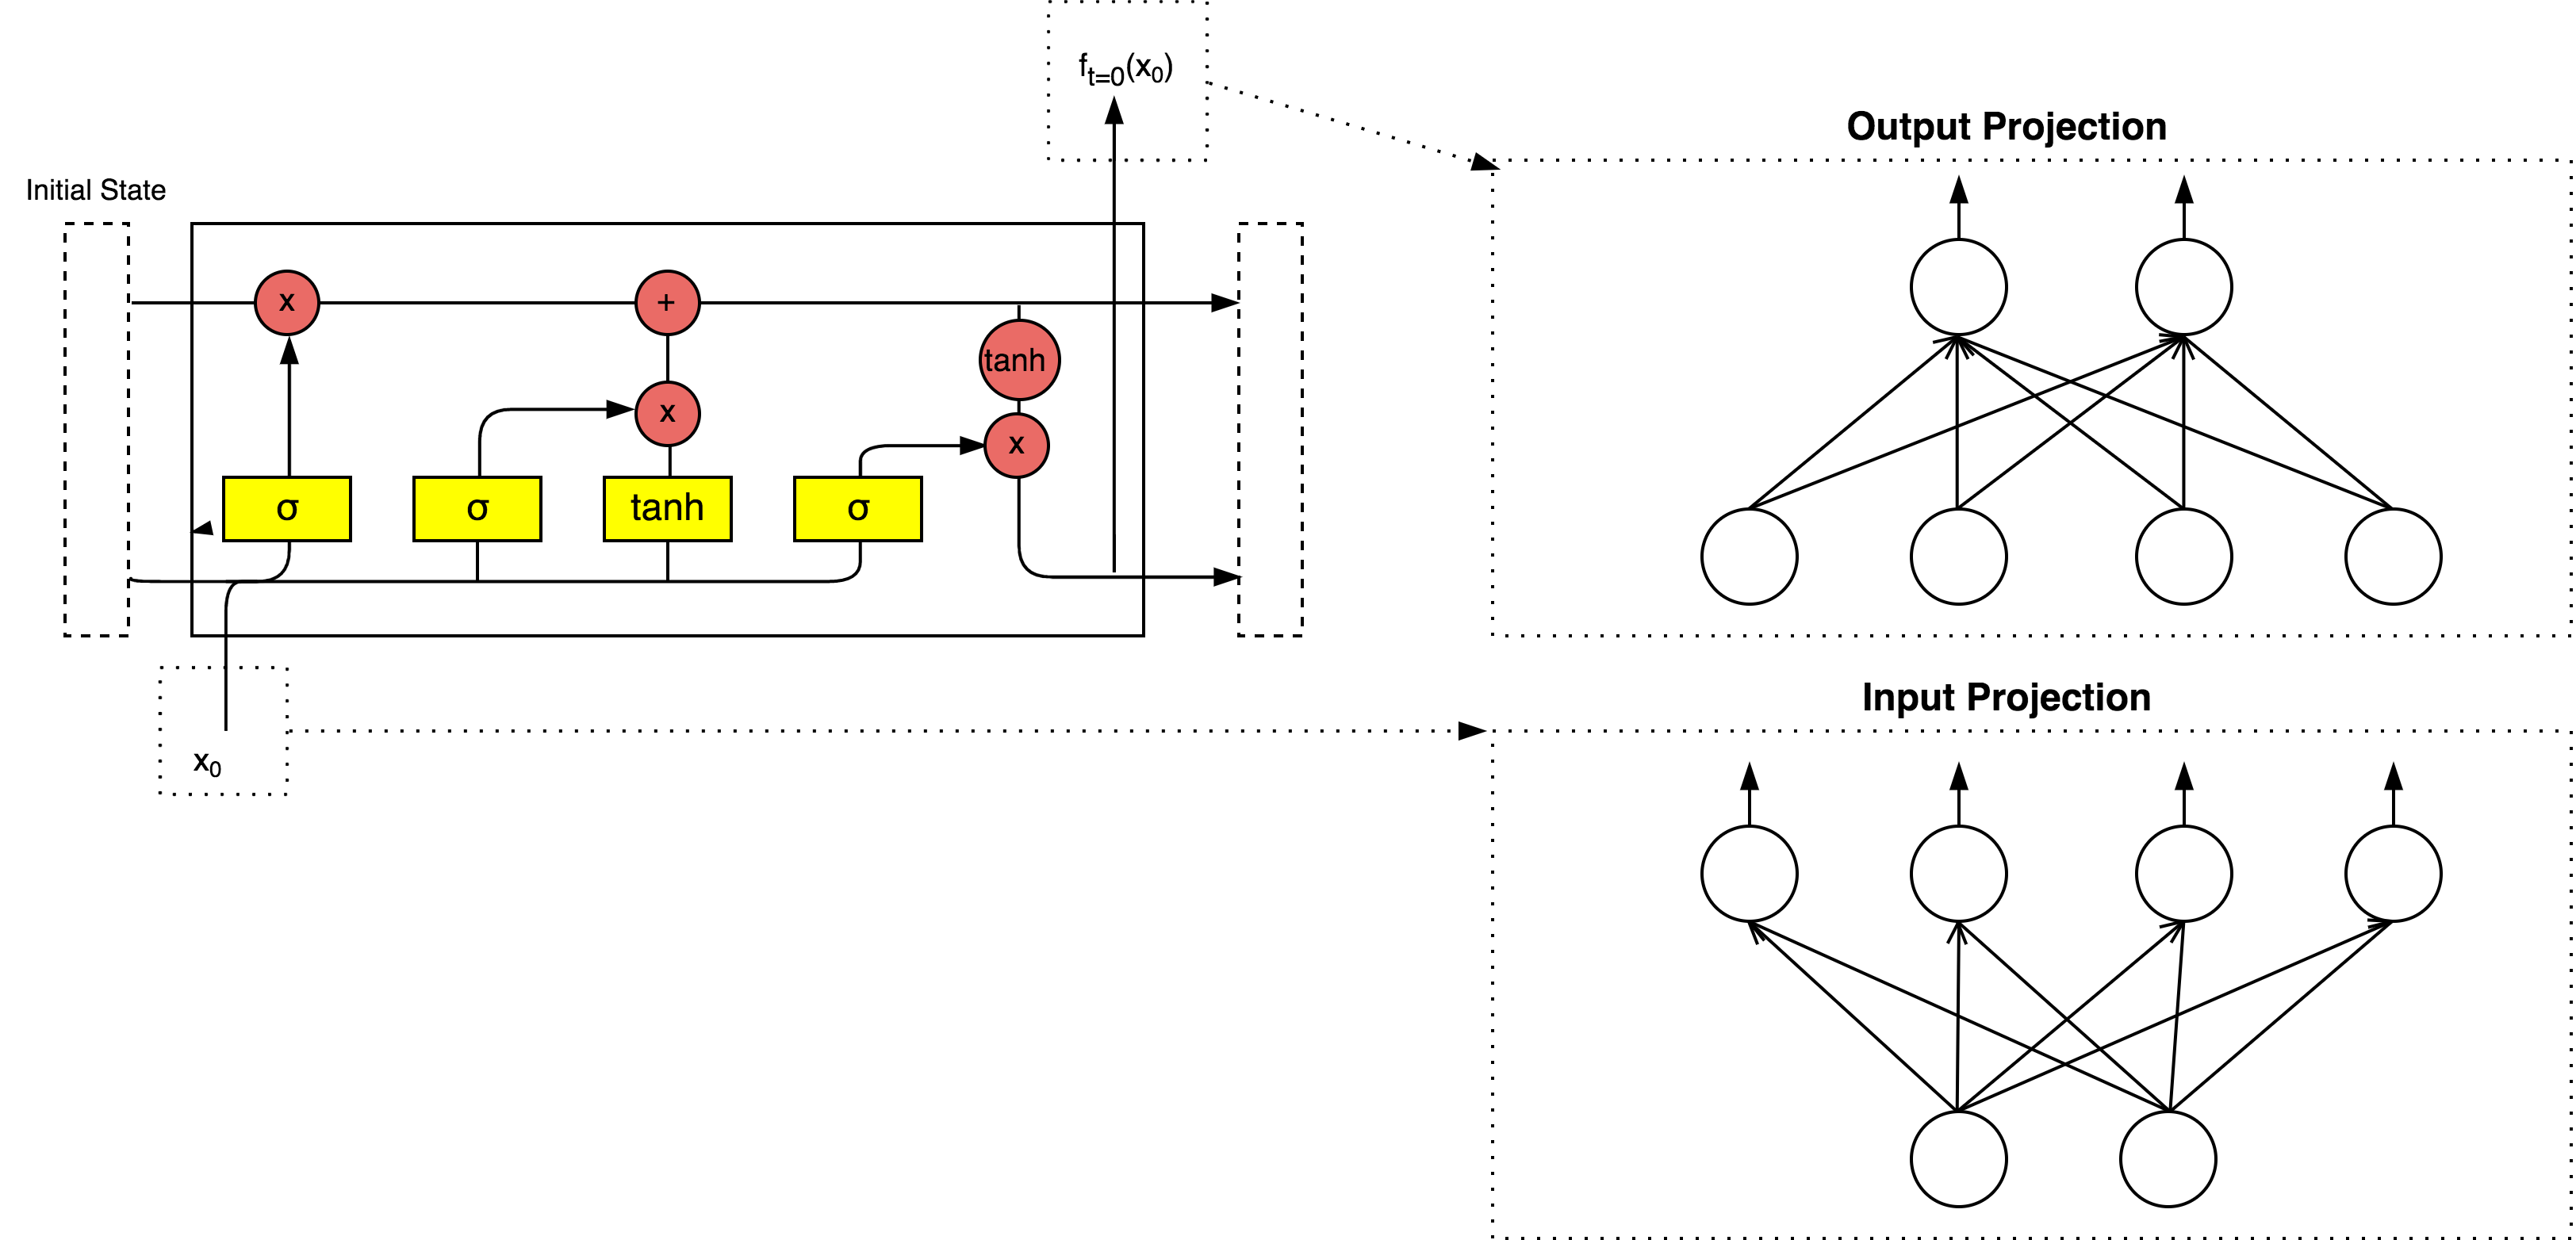
\includegraphics[width=0.7\textwidth]{lstm-projection}
  \caption{Example of projection within a LSTM cell with 4 hidden states.}
  \label{fig:lstm-projection}
\end{figure}

\newpage

Some of the traces can be particularly long and therefore the network needs to be unrolled to extreme lengths \cite{greschbach2016effect}.
In fact, given memory constraints, this becomes a major problem.
But it can be solved by cutting the traces after a couple seconds since it has been shown that the first part of a trace carries more information than the latter.

\begin{figure}[ht]
  \centering
  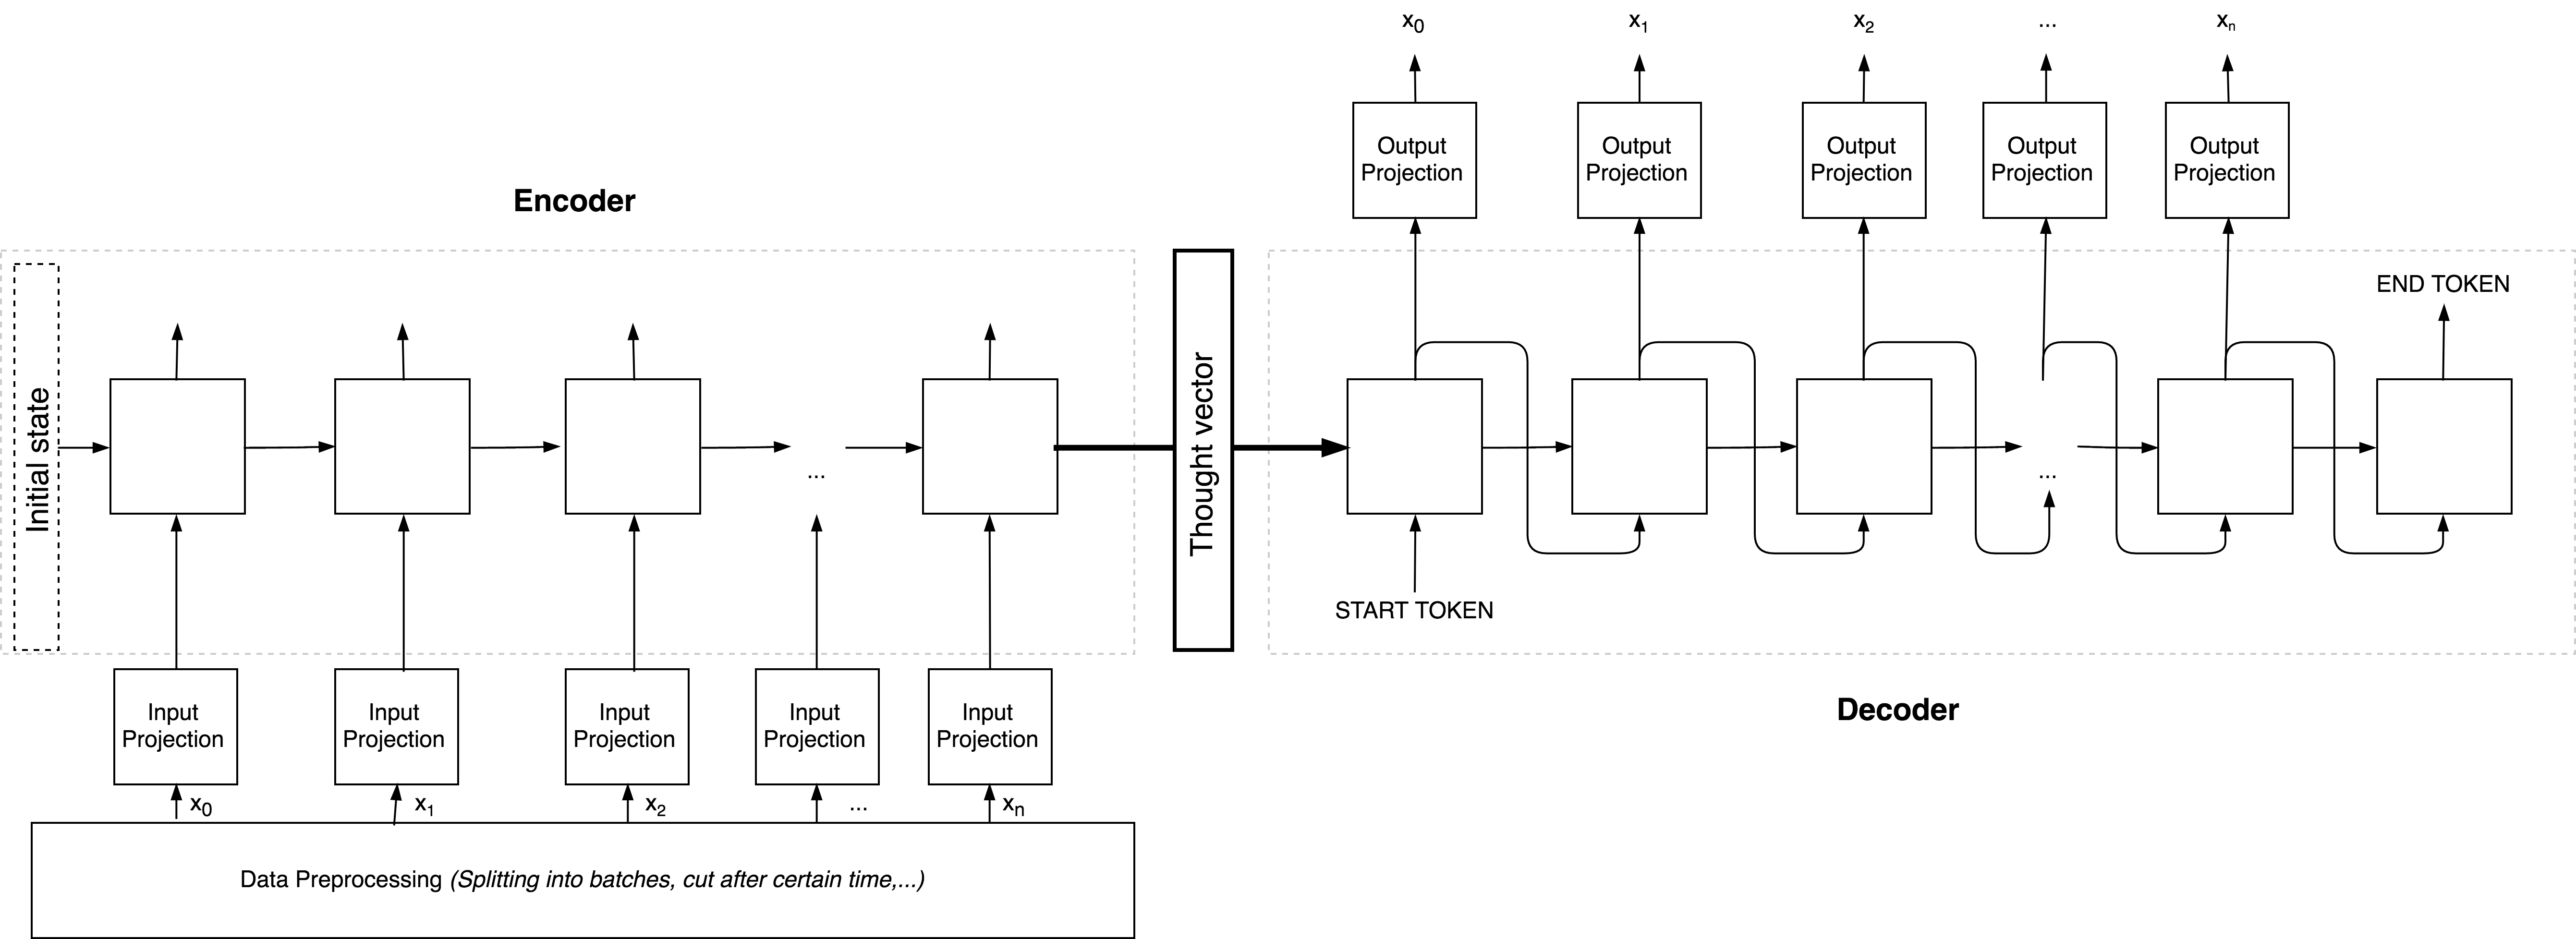
\includegraphics[width=\textwidth]{full-seq2seq}
  \caption{Overal structure of our sequence-to-sequence model.}
  \label{fig:full-seq2seq}
\end{figure}

Based on the above, we can construct our \textit{computational graph} in Tensorflow as outlined in figure \ref{fig:full-seq2seq}.

\section{Attack Strategy}

Here we consider an adversary that relies on deep learning to extract fingerprints for a website fingerprinting attack.
This adversary can have two different goals in mind, as previously stated in section \ref{sec:threat-model}.
The full attack, however, can be split up into four different stages, namely \textit{data collection}, \textit{fingerprint extraction training}, \textit{classifier training} and \textit{the attack}.

\noindent
\textbf{Data Collection}
\begin{enumerate}
  \item Choose web pages that the attacker wishes to monitor.
  \item Collect traffic for a set of monitored and unmonitored sites.
  \item Convert the raw TCP data into Tor cells.
  \item Remove SENDMEs and other noise.
\end{enumerate}

\noindent
\textbf{Fingerprint Extraction Training}
\begin{enumerate}[resume]
  \item Further process the data into batches and perform any other preprocessing required by the model such as cutting or padding the traces.
  \item Prepare the fingerprint extraction model.
  \item Train the fingerprint extraction model on a copy task for monitored and some unmonitored web pages.
  \item Extract fingerprints from data by using the trained model.
\end{enumerate}

\noindent
\textbf{Classifier Training}
\begin{enumerate}[resume]
  \item Given a classifier, train it using the extracted fingerprints.
  \item Measure performance of classifier.
\end{enumerate}

\noindent
\textbf{The Attack}
\begin{enumerate}[resume]
  \item Passively capture traffic from Tor users.
  \item Pre-process the collected data.
  \item Extract fingerprints using the trained fingerprint extraction model.
  \item Classification via the trained classifier.
\end{enumerate}

\begin{figure}[ht]
  \centering
  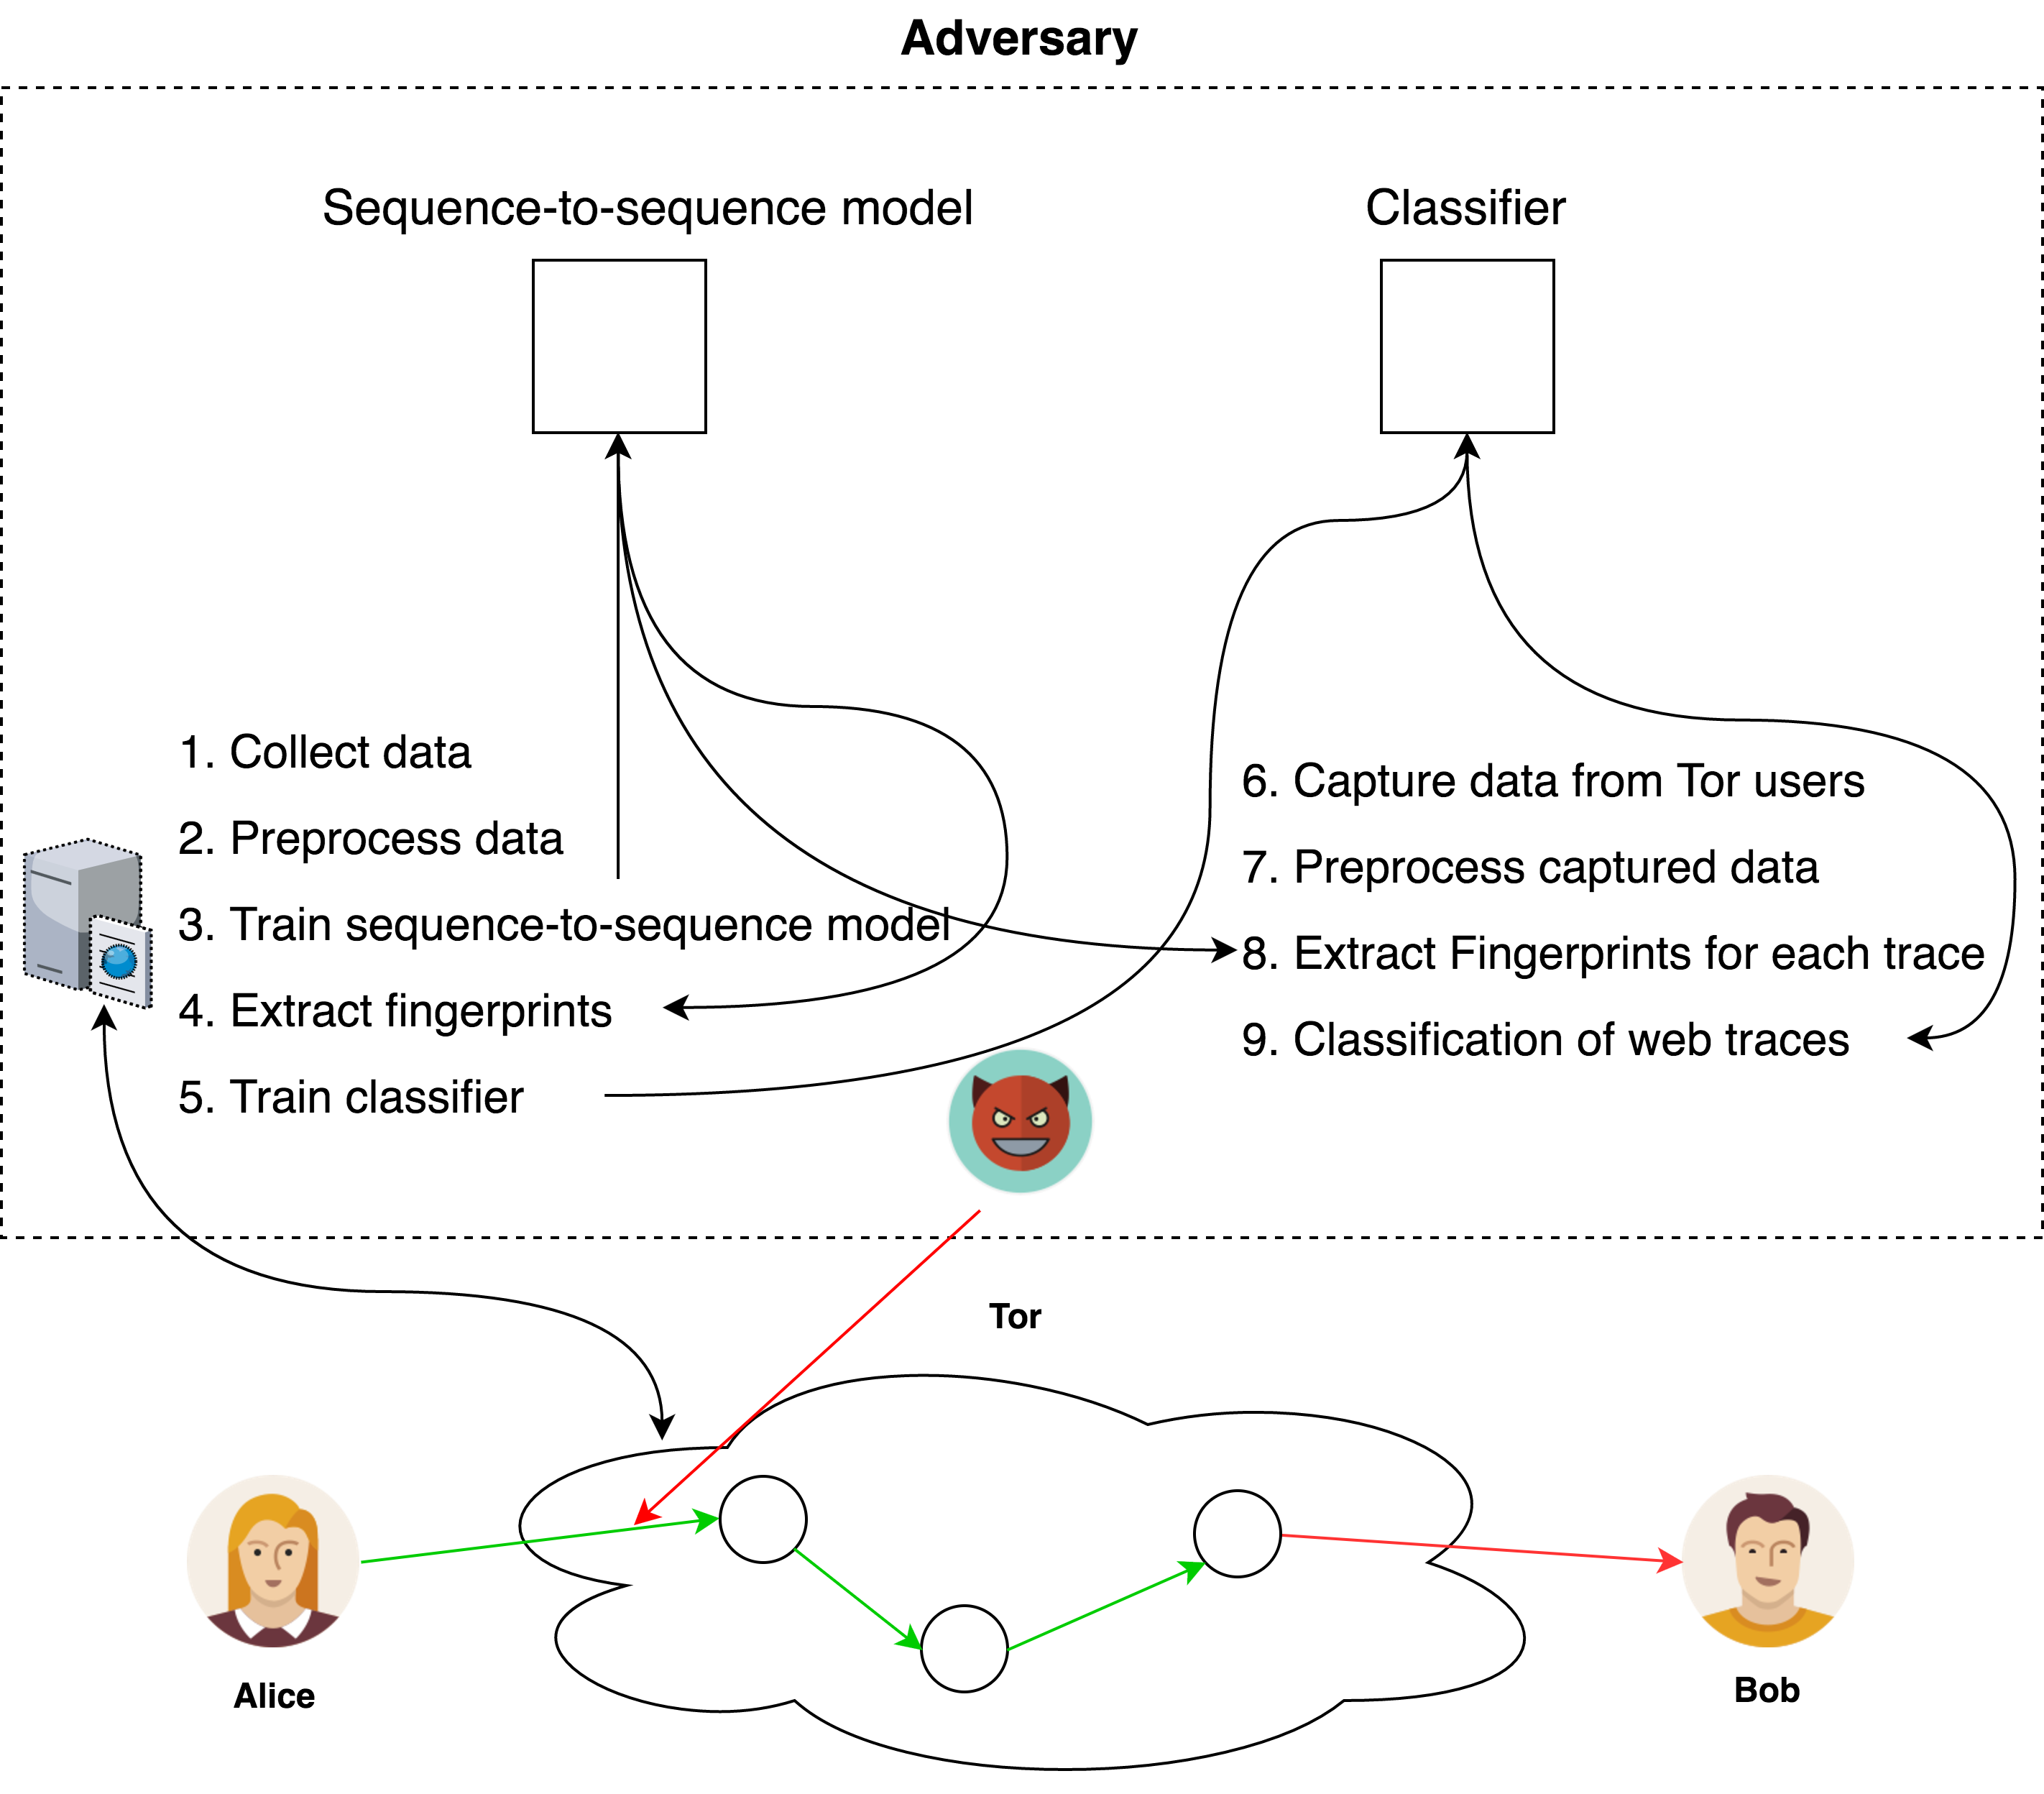
\includegraphics[width=0.7\textwidth]{overall-structure}
  \caption{Attack strategy.}
  \label{fig:attack-strategy}
\end{figure}

\subsection{Data Collection} \label{sec:data_collection1}

As previously mentioned, the data collection process first requires the adversary to choose a set of $n$ websites to monitor.
Next, the adversary crawls these pages a total of $i$ iterations to ensure that a classifier has enough data to generalize.
As suggested by Wang et al. when performing page loads, browser caching should be disabled since Tor does not allow caching to disk and therefore the browser cache should be cleared every time a web page is loaded\cite{wang_goldberg_2013}.
After the collection, the TCP data is converted into Tor cells and probabilistic algorithms are used by Wang et al. \cite{wang_goldberg_2013} to remove SENDMEs.
This data can be processed further, however we chose not to since the model should be able to learn how to perform this processing.

Most of our analysis will be done using the dataset provided by Greschbach et al. \cite{greschbach2016effect}, which can be used for open-world analysis since it provides us with $100$ samples for Alexa's top $9000$ websites and one sample of one sample for $909,000$ unmonitored sites.
For the rest of this paper, we will refer to this dataset as \texttt{GRESCHBACH}.
Next, to see how our model performs on a dataset, whose data is recorded at a different time and under different circumstances, we will also be using the dataset provided by Wang et al. \cite{wang_cai_johnson_nithyanand_goldberg_2014}, which we will call \texttt{WANG14} \cite{panchenko2}.
This set is slightly smaller with $100$ monitored websites with $90$ instances each and $8400$ unmonitored sites.

\subsection{Fingerprint Extraction Training} \label{sec:fingerprint-extraction-training}

In order to truly evaluate the model, we need to split the data up into a training and validation set.
We do not train the model on any data in the validation set but instead use it to see how well the model performs on unseen data.
For this split, we use a \textit{stratified shuffle split}, meaning that we shuffle the data and then perform the split, whilst preserving the class distributions.
On top of training the feature extractor with monitored pages, we also train it on unmonitored pages, as it needs to be able to extract features effectively from both sets.

During training and extracting the fingerprints, \textit{mini-batch processing} will always be used.
This will allow us to gain a performance boost and perhaps even have a faster convergence.
When dividing the data up into these batches, we also need to determine how big they will be.
The bigger they are, the larger the performance gain will be but the lower the accuracy might be.
Additionally, the size of the batches also depend on the amount of available memory since we cannot have the VM run out of memory whilst training.

On top of determining the batch size, the individual models require different preprocessing steps and tuning of different parameters.

\subsubsection{Stacked Autoencoder}

As previously mentioned, after dividing the data up into batches, we either need to cut or pad the traces such that they all are of a fixed-length.
Next, we know that the first layer needs to have the same amount of neurons than the length of the input.
But after that, there are a variety of different architectures that need to be chosen.
Some of which are outlined below:

\newpage

\begin{itemize}
  \item How many hidden layers we want.
    The more there are, the more complex the functions are that the model can learn but the harder it becomes to train the model.

  \item The amount of hidden neurons in each layer.
    This number should gradually decrease to the number of features we would like to extract.

  \item The activation function of the neurons.
    The most popular ones being \textit{sigmoid}, \textit{ReLu} and an \textit{atan}.

  \item Whether or not to include batch normalization at every step.
\end{itemize}

Now that the model has been constructed, there are still several learning parameters that need to be tuned:

\begin{itemize}
    \item The optimizer to use (\textit{adam}, \textit{gradient descent} or \textit{RMSProp}) \cite{tensorflow}.
    \item Learning rate ($\gamma$) for the previously chosen optimizer.
    \item Amount of traces within a single mini-batch ($b$).
    \item Cost, or loss function ($f$) to minimize (\textit{mean squared error} (MSE), \textit{absolute loss} (AL) or \textit{cross-entropy}) \cite{tensorflow}.
\end{itemize}

\subsubsection{Sequence-to-Sequence Model}

Each batch can either be presented in \textit{batch-major} or \textit{time-major} form.
Although time-major is slightly more efficient \cite{tensorflow}, we opt for a batch-major form, since it makes the fingerprint extraction process easier.
Next, after the data has been divided into mini-batches, we perform some further processing such as cutting the traces after several seconds.
Finally, since all of the traces within a batch need to be of the same length, padding is performed as a final preprocessing step.

After collecting and fully preprocessing the data, the adversary can start to construct the sequence-to-sequence model.
However, in order to do so, there are a variety of different architectures that need to be considered, some of which are outlined below:

\begin{itemize}
  \item Which sort or RNN cells to use. This can either be a GRU or an LSTM cell.
    We could also potentially investigate the usefulness of multilayered RNN cells but we expect the performance gain to be very limited.

  \item Using a bidirectional encoder to ensure that the output at time $t$ is not only affected by past information but also on future information.

  \item The amount of hidden states within a RNN cell, which affects the size of the fingerprints.
\end{itemize}

Now that the model has been constructed, the adversary still has to chose various learning parameters such as:

\newpage

\begin{itemize}
  \item The optimizer to use (\textit{adam}, \textit{gradient descent} or \textit{RMSProp}) \cite{tensorflow}.
  \item Learning rate ($\gamma$) for the previously chosen optimizer.
  \item Amount of traces within a single mini-batch ($b$).
  \item Cost, or loss function ($f$) to minimize (\textit{mean squared error} (MSE), \textit{absolute loss} (AL) or \textit{cross-entropy}) \cite{tensorflow}.
  \item After how much time the traces are cut.
\end{itemize}

After these parameters have been tuned, the computational graph can be constructed in Tensorflow and the model can be trained.
When this training has been completed, fingerprints can finally be extracted for all the traces in the test set.

\subsection{Classifier Training} \label{sec:classifier-training}

When the adversary has extracted the fingerprints for websites within the test set, they need to train a classifier.
Most works so far rely on some sort of \textit{supervised machine learning} techniques such as \textit{support vector classifiers} (SVC), \textit{k-nearest neighbours} (kNN), \textit{random forests} (RF) or \textit{naive bayes} (NB) \cite{panchenko1,panchenko2,wang_cai_johnson_nithyanand_goldberg_2014,kfingerprinting,naivebayes}.
All of these algorithms rely on different techniques but an explanation of their inner workings is outside the scope of this paper.
Instead, we will consider them as \textit{black box models}.
This means that all we know is that we can apply a \texttt{fit} function to the models, which causes them to learn how to classify the fingerprints and a \texttt{predict} function, which predicts the classes of given inputs.

To measure the performance of our black-box models, we use a similar technique as we did in the previous section.
We split our test set up into two more sets, a \textit{classifier training set} and a \textit{classifier test set}.
But since training a classifier, requires less time, we can use another technique, called \textit{stratified k-fold validation}.
Here we split our original test set up into $k$, mutually exclusive, folds.
Next, one of the folds is chosen to be the classifier test set and all of the other folds form the classifier training set.
This process is repeated for $k$ iterations, where for each iteration, a different fold is chosen to be a test set.
But again, we preserve the class distributions within all of the folds.

\begin{figure}[ht]
  \centering
  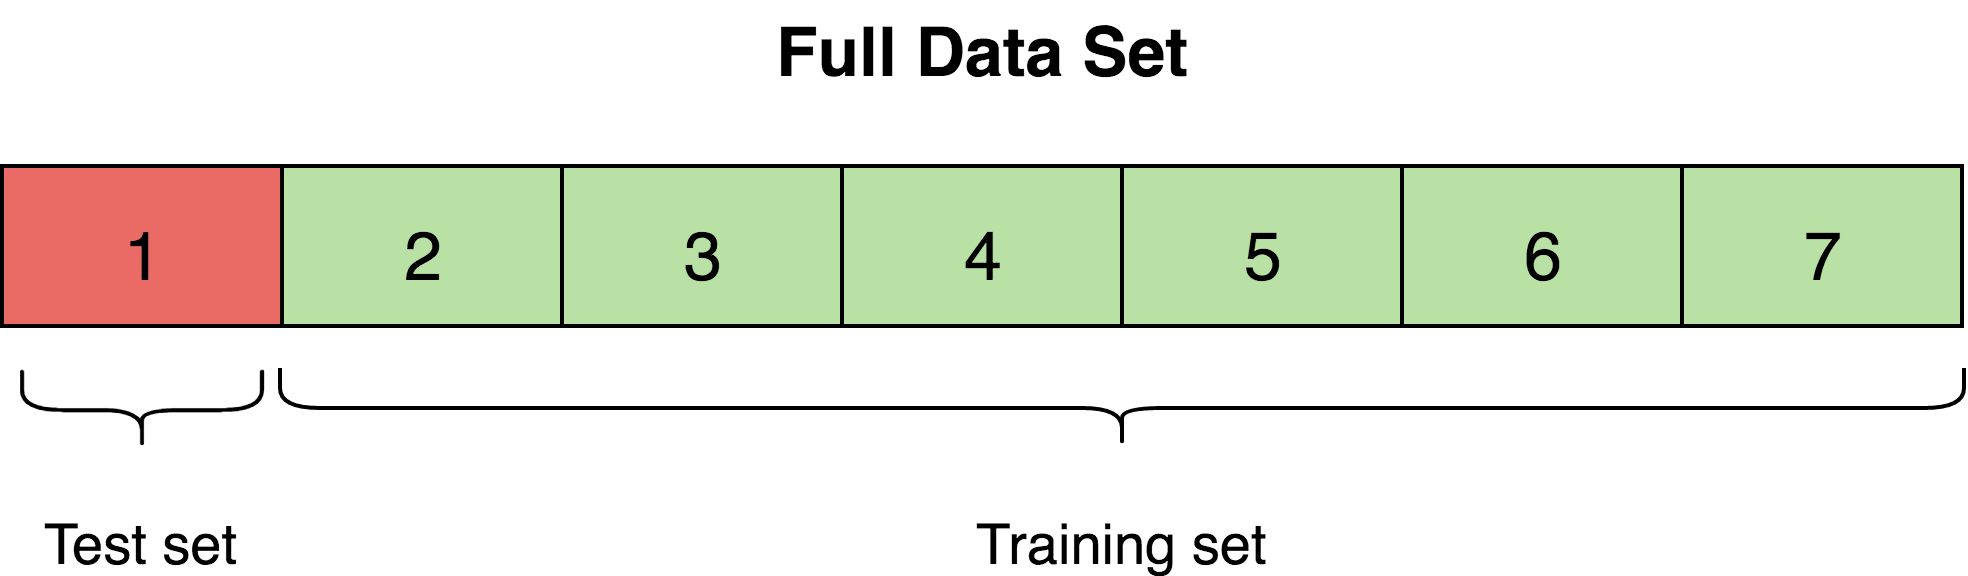
\includegraphics[width=0.6\textwidth]{kfold}
  \caption{Example of one iterations in a k-fold validation $(k = 7)$.}
  \label{fig:kfold}
\end{figure}

For each iteration of the validation process, several statistics can be recorded and then averaged over all iterations.
The k-fold validation process ensures that every data point will be in the test set at least once and therefore giving us an accurate measure of these statistics.

Some of the performance measures that we will use in the evaluation stage are outlined below within the context of a WF attacks:
\begin{itemize}
  \item \textbf{True Positive Rate (TPR)} is the probability that a monitored page is classified as the correct monitored page \cite{kfingerprinting}.

  \item \textbf{False Positive Rate (FPR)} is the probability that an unmonitored page is incorrectly classified as a monitored page \cite{kfingerprinting}

  \item \textbf{Bayesian Detection Rate (BDR)} is the probability that a page corresponds to the correct monitored page, given that the classifier recognized it as that monitored page \cite{kfingerprinting}.
    This can be calculated as follows:
    $$\text{BDR} = \frac{\textit{TPR} \times \Pr(M)}{\textit{TPR} \times \Pr(M) + \textit{FPR} \times \Pr(U)}$$
    where
    $$\Pr(M) = \frac{|\text{Monitored}|}{|\text{Total Pages}|}, \quad \Pr(U) = 1 - \Pr(M)$$

    This measure essentially indicates the practical feasibility of the attack, as the adversary is mainly concerned with this specific measure \cite{kfingerprinting}.

  \item \textbf{Accuracy (A)} is the percentage of correctly classified instances.
    Although it can be used as a rough indicator, it will not be used in the final conclusions because of the \textit{accuracy paradox}, which arises due to class imbalance.

  \item \textbf{F1-Score (F1)} measures the harmonic mean between precision and recall \cite{scikitlearn}.
    \begin{align*}
      \text{F1} &= 2 \times \frac{\text{precision} \times \text{recall}}{\text{precision} + \text{recall}}\\
                &= \frac{2 \times \textit{TP}}{2 \times \textit{TP} + \textit{FP} + \textit{FN}}
    \end{align*}
    where
    $$\text{recall} = \frac{\textit{TP}}{\textit{TP} + \textit{FN}}, \quad \text{precision} = \frac{\textit{TP}}{\textit{TP} + \textit{FP}}$$

    This measure is particularly useful since it is not affected by class imbalance.
\end{itemize}

Rather than using another classifier, we could potentially add a \textit{softmax layer} on top of our encoder, like V. Rimmer uses on top of her stacked autoencoder \cite{deeplearningthesis}.
We could use this idea for both our autoencoder and the sequence-to-sequence model.

This process would involve first training the sequence-to-sequence model, then stacking the softmax layer on top of each unrolled cell in the encoder and using it for classification.
What would be interesting about this approach is that the adversary can analyse how certain the classifier is, as it analyses packets more and more packets from the trace.
However, this is outside the scope of this paper, as we are focusing on the feature extraction process.

\begin{figure}[ht]
  \centering
  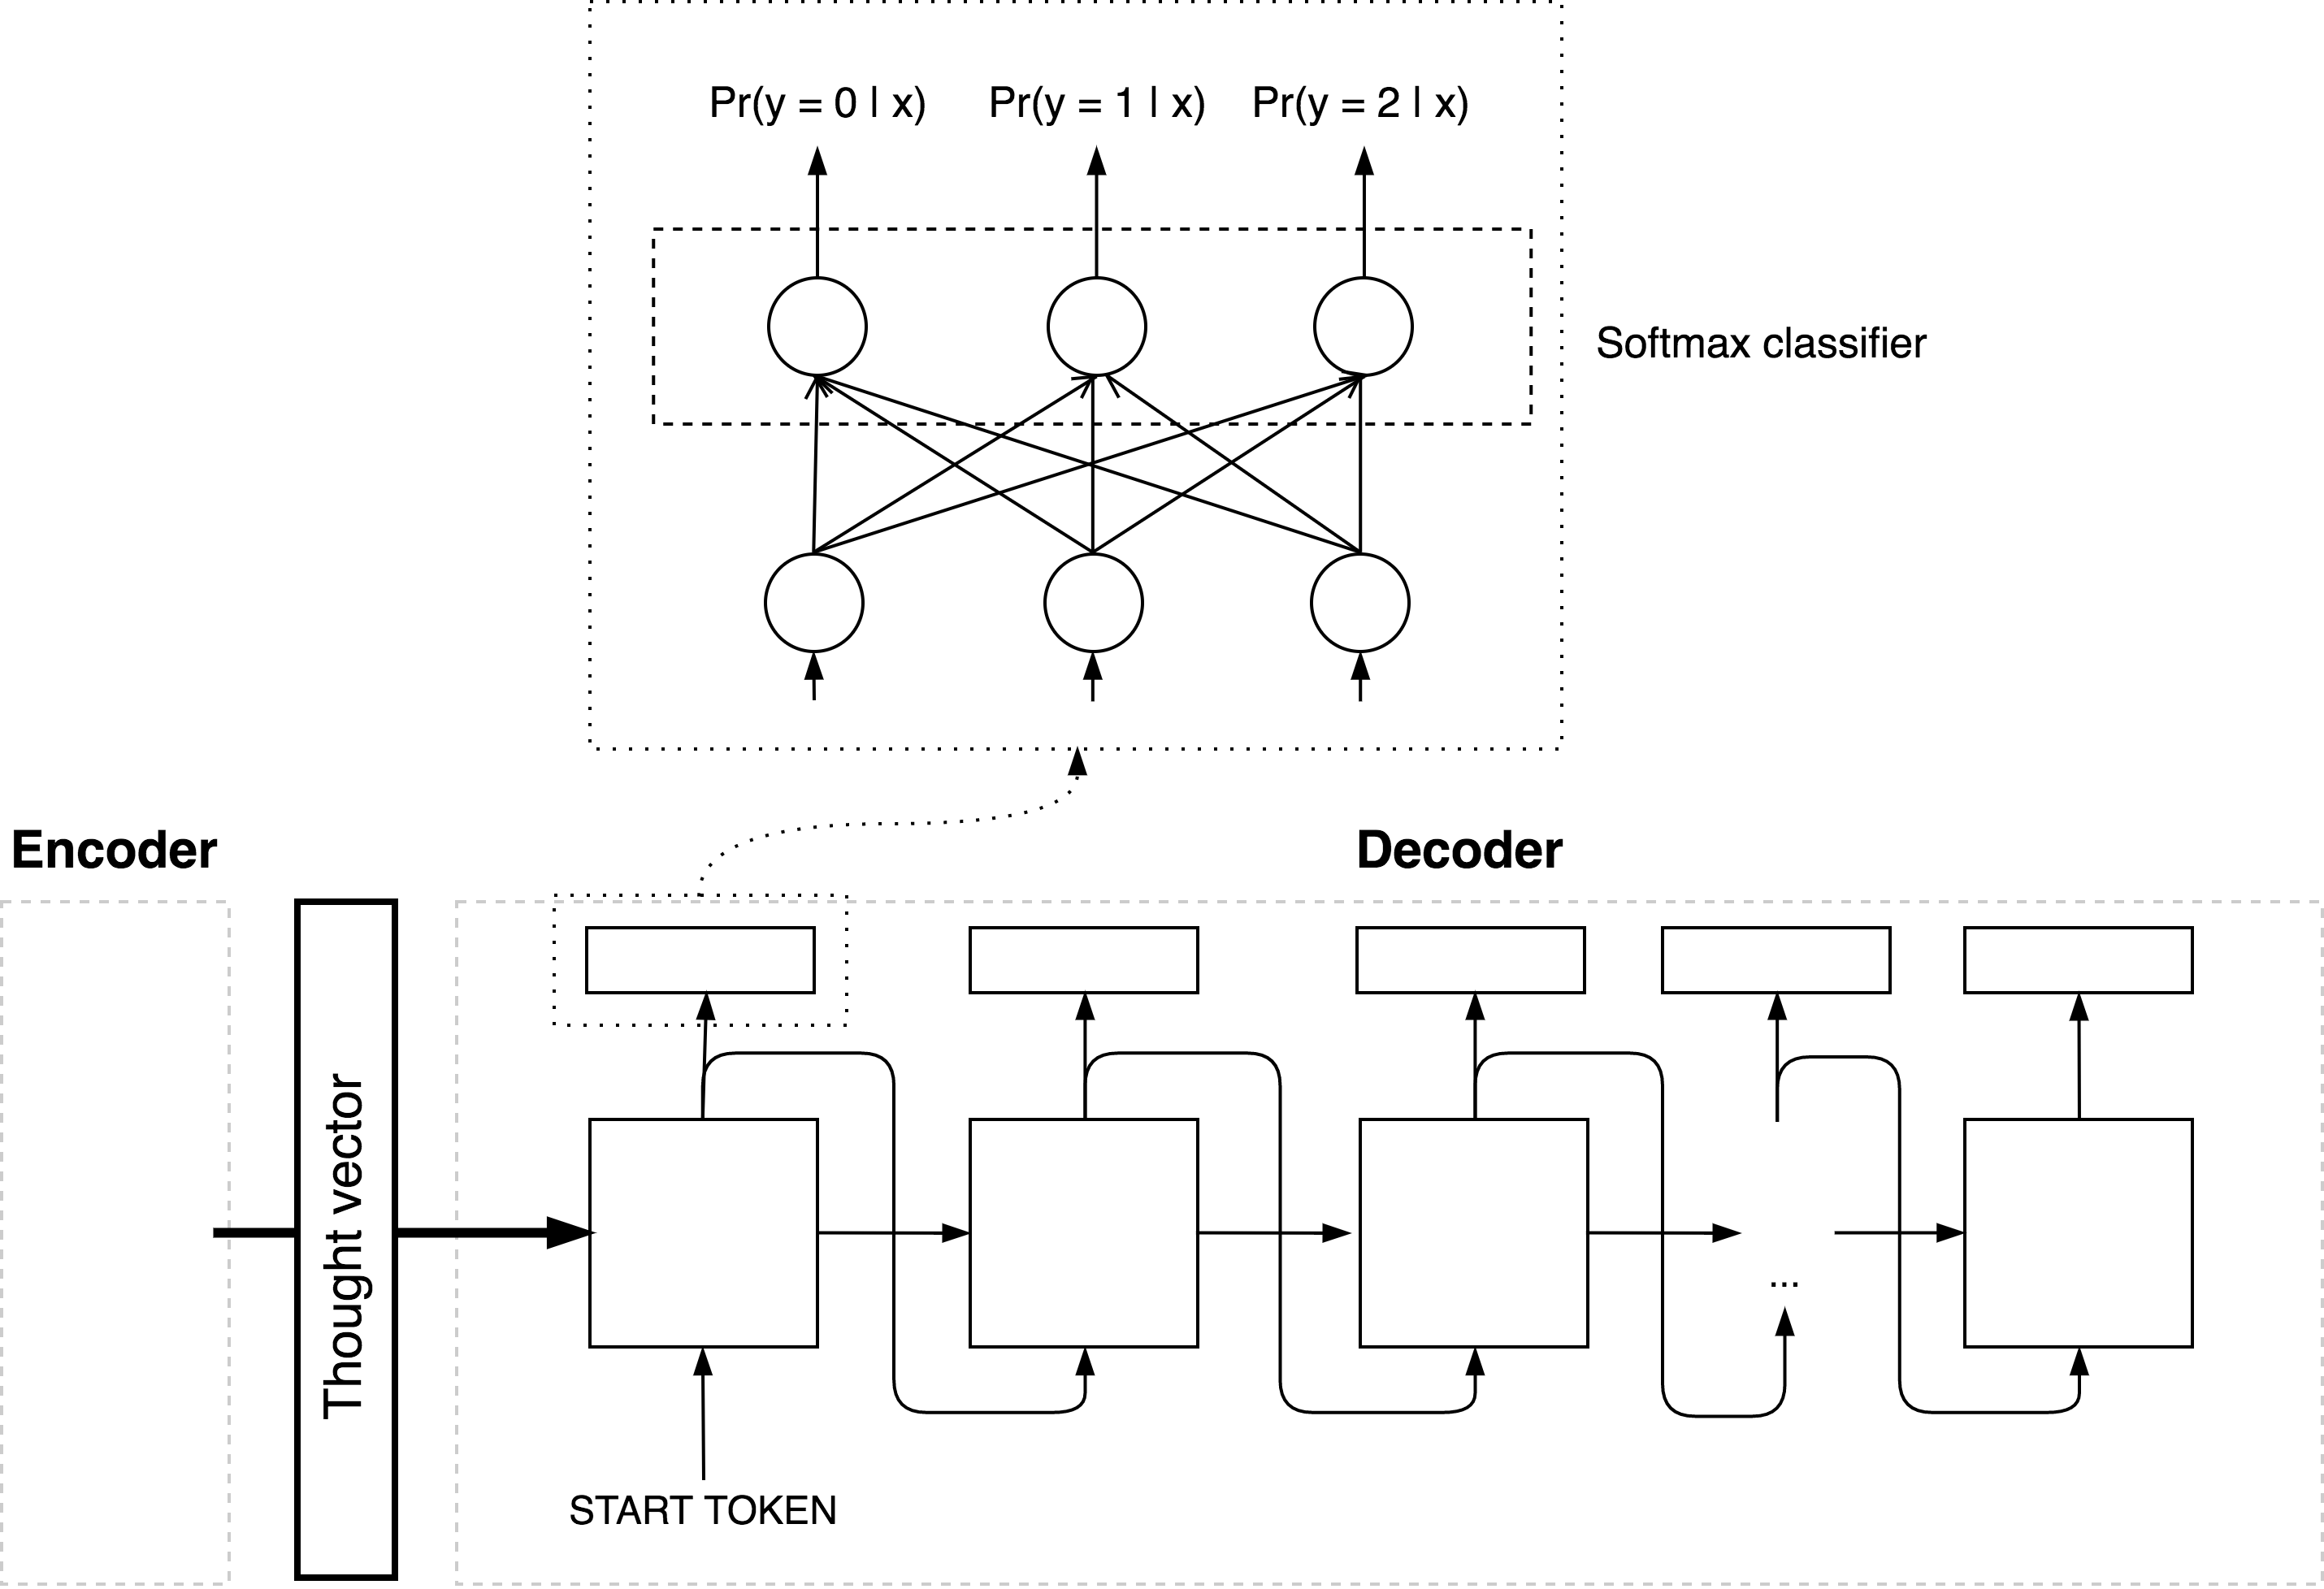
\includegraphics[width=0.55\textwidth]{softmax}
  \caption{Example of encoder with softmax layer for 3 web pages.}
  \label{fig:softmax}
\end{figure}

\newpage

\subsection{The Attack}

Finally, after the adversary has trained the required models, the real WF attack can start.
First, the adversary starts capturing web traffic data between the user and the entry guard, as shown in figure \ref{fig:threat_model}.
Next, the data is processed for the fingerprint extraction process, as described in section \ref{sec:fingerprint-extraction-training}.
After all the processing has finished, fingerprints are extracted using the previously trained model.
Finally, those fingerprints are used as features for a classifier, which classifies the traffic into web pages.

The time between data collection for training and performing the WF has to be kept as small as possible since Juarez et al.'s experiments show that website's content changes greatly over time, therefore affecting the accuracy of the attack \cite{wfpevaluation}.

\section{Code Structure} \label{sec:code-structure}

In the work, we will not be conducting the final stage of a WF attack.
Instead, we will be reporting the results on the test sets.
All of this is reflected in the overall structure of the code, which consists of four main components, as can be seen in figure \ref{fig:code-structure}.

\begin{figure}[ht]
  \centering
  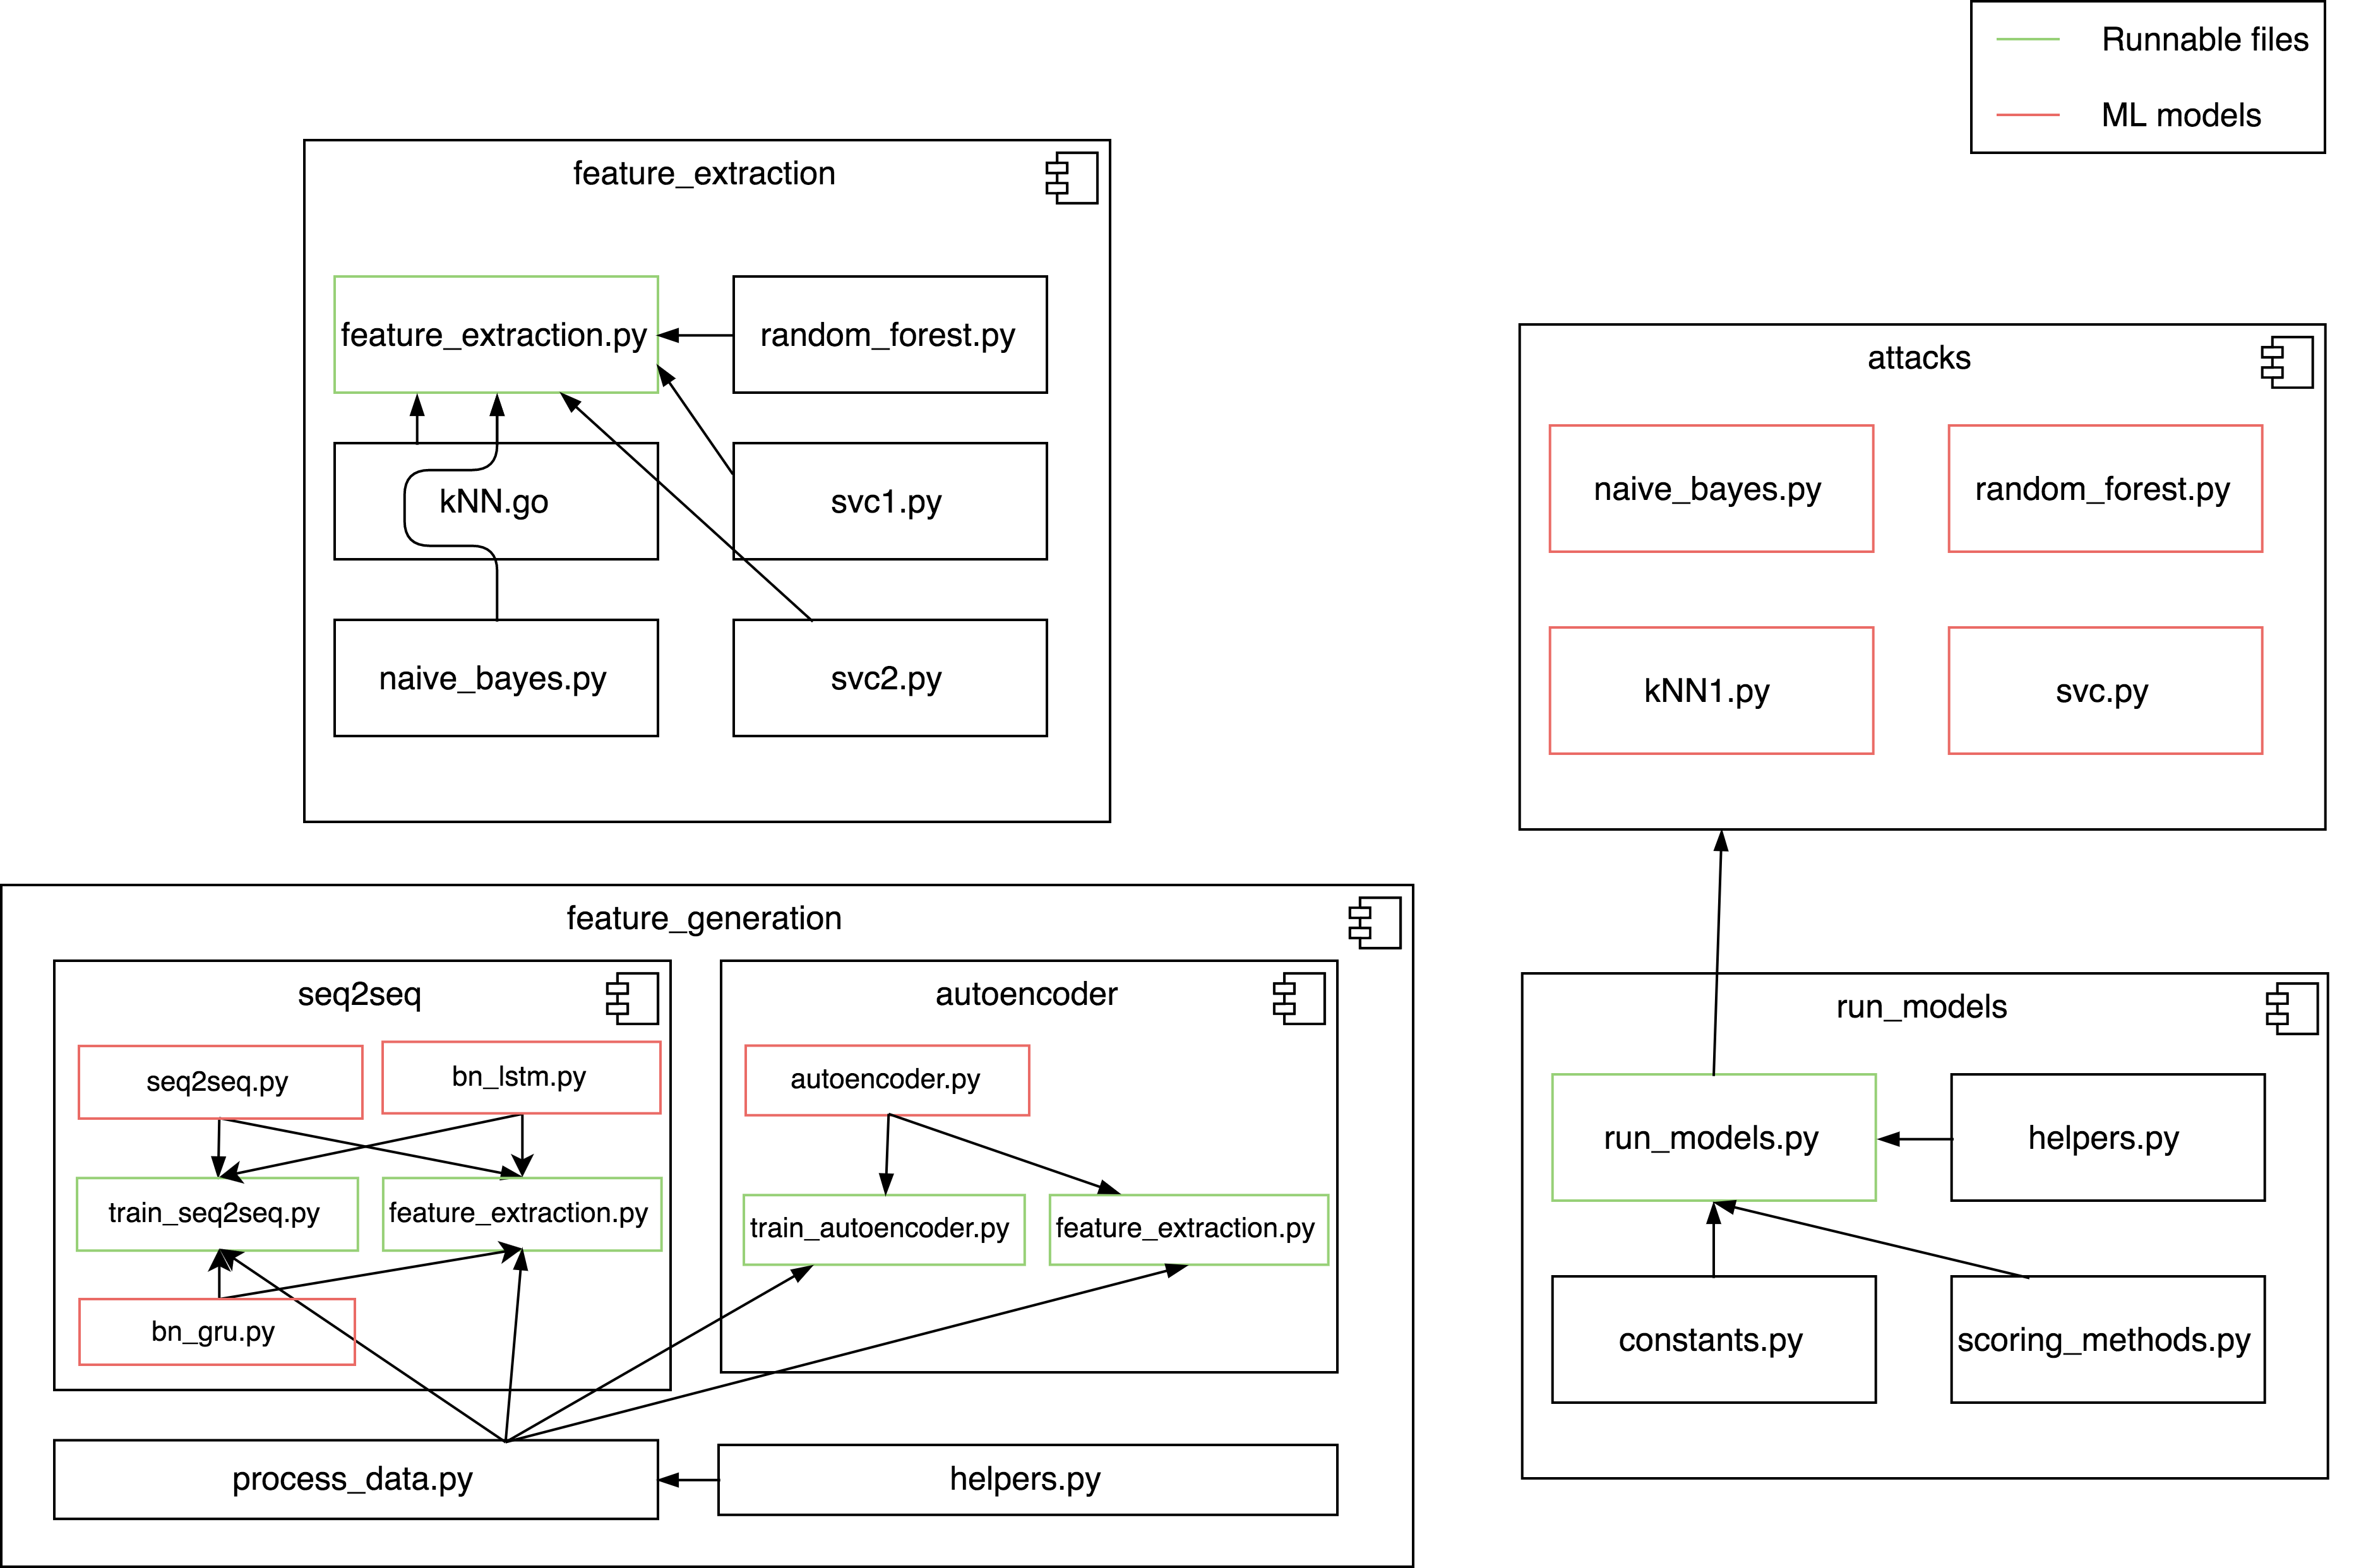
\includegraphics[width=\textwidth]{code-structure}
  \caption{Diagram of how different components are related.}
  \label{fig:code-structure}
\end{figure}

All of the data that is used within this work has already been preprocessed into Tor cells with SENDMEs removed, as described in section \ref{sec:data_collection1}.
The \texttt{feature\_generation} module contains all of the code to further preprocess the data, train the fingerprint extraction models and to extract the fingerprints using the respective model.

The classifiers that will be used for the attacks are defined in the \texttt{attacks} module.
We tried to pick a variety of existing models to measure how our extracted fingerprints work on different classifiers.
The logic to actually test the attacks is defined in the \texttt{run\_models} module, which also does some data preprocessing, defines the logic for the stratified k-fold validation and the different scoring methods.

\newpage

Finally, there is also the \texttt{feature\_extraction} module, whose use will be explained later.

As can be seen, all of the code is written in Python, due to the wide availability of machine learning tools.
Except for the \texttt{kNN.go} file, in the \texttt{feature\_extraction} module, which is written in \textit{Golang} to gain a performance boost \cite{gokNN}.
